\documentclass[14pt]{extarticle}

\usepackage{fontspec}
\setmainfont{Times New Roman}

% размер полей
\usepackage{geometry}
\geometry{a4paper, top=2cm, bottom=2cm, right=1.5cm, left=3cm}

 %debugging
%\usepackage{showframe}

% полуторный интервал
\usepackage{setspace}
\onehalfspacing

% абзацный отступ
\setlength{\parindent}{1.25cm}

% выравнивание текста по ширине
\sloppy

% списки
\usepackage{calc} % арифметические операции с величинами
\usepackage{enumitem}
\setlist{
    nosep,
    leftmargin=0pt,
    itemindent=\parindent + \labelwidth - \labelsep,
}

% подписи к рисункам и таблицам
\usepackage{caption}
\renewcommand{\figurename}{Рисунок}
\renewcommand{\tablename}{Таблица}
\DeclareCaptionFormat{custom}
{
    \textit{#1#2#3}
}
\DeclareCaptionLabelSeparator{custom}{. }
\captionsetup{
    % хз какой это размер - 12 или нет, но выглядит меньше 14
    font=small,
    format=custom,
    labelsep=custom,
}

% картинки
\usepackage{graphicx}

% колонтитулы
\usepackage{fancyhdr}

% картинки и таблицы находятся именно в том месте текста где помещены (атрибут H)
\usepackage{float}

% таблицы
\usepackage{tabularray}

\graphicspath{ {4.2.2/models/} }
\begin{document}
\pagestyle{fancy}
\fancyhead{}
% disable header
\renewcommand{\headrulewidth}{0pt}
\fancyfoot[L]{Дубровских гр 221-361}
\fancyfoot[C]{ЛР 4.2.2}
\fancyfoot[R]{Продажа автотранспорта}
\singlespacing

\newpage
\begin{center}
    Министерство науки и высшего образования Российской Федерации
    Федеральное государственное автономное образовательное учреждение

    высшего образования

    \guillemotleft МОСКОВСКИЙ ПОЛИТЕХНИЧЕСКИЙ УНИВЕРСИТЕТ\guillemotright

    (МОСКОВСКИЙ ПОЛИТЕХ)
\end{center}
\noindent
\bigbreak
\bigbreak
\bigbreak
\bigbreak
\begin{center}
    ЛАБОРАТОРНАЯ РАБОТА 4.2.2

    По курсу Проектирования пользовательских интерфейсов в веб

    \textbf{Проектирование взаимодействия экранов (Wire flow)}
    \bigbreak
    \bigbreak
    \bigbreak
    \bigbreak
    ТЕМА

    \guillemotleft\textbf{САЙТ ДЛЯ ПРОДАЖИ И ПОИСКА АВТОМОБИЛЕЙ}\guillemotright
\end{center}
\noindent
\bigbreak
\bigbreak
\bigbreak
\bigbreak
\bigbreak
\bigbreak
\bigbreak
\bigbreak
\bigbreak
\bigbreak
\hfill Выполнил

\hfill Дубровских Никита Евгеньевич

\hfill Группа 221-361
\bigbreak
\bigbreak
\bigbreak
\hfill Проверил

\hfill Натур ВВ
\vfill
\begin{center}
    Москва, 2024
\end{center}
\newpage
\onehalfspacing


\begin{center}
    \textbf{Лабораторная работа 4.2.2}

    \textbf{Проектирование взаимодействия экранов (Wire flow)}
\end{center}

\textbf{Цель работы:} связать элементы на экранах/страницах в логические цепочки взаимодействия 
\bigskip

\textbf{Задачи:}

\begin{enumerate}
    \item Определить взаимосвязи между элементами страниц.
    \item Добавить к варфреймам пути взаимодействия их элементов.
\end{enumerate}
\bigskip

\textbf{Основные термины}

\begin{itemize}
    \item Wire flow - объединение блок-схемы и каркасов, документирующее рабочий процесс и дизайн экрана с несколькими динамически меняющимися страницами.
    \item Блок-схемы - графическое представление процесса или системы, показывающее взаимосвязи между элементами.
    \item Потоки задач (Task Flow) - последовательность действий, которые пользователь выполняет для достижения цели.
    \item Мудборды - визуальные коллажи, представляющие идеи и концепции дизайна.
\end{itemize}
\bigskip

\textbf{Wireflow}
\bigskip

\noindent
\begin{minipage}{\linewidth}
    \fbox{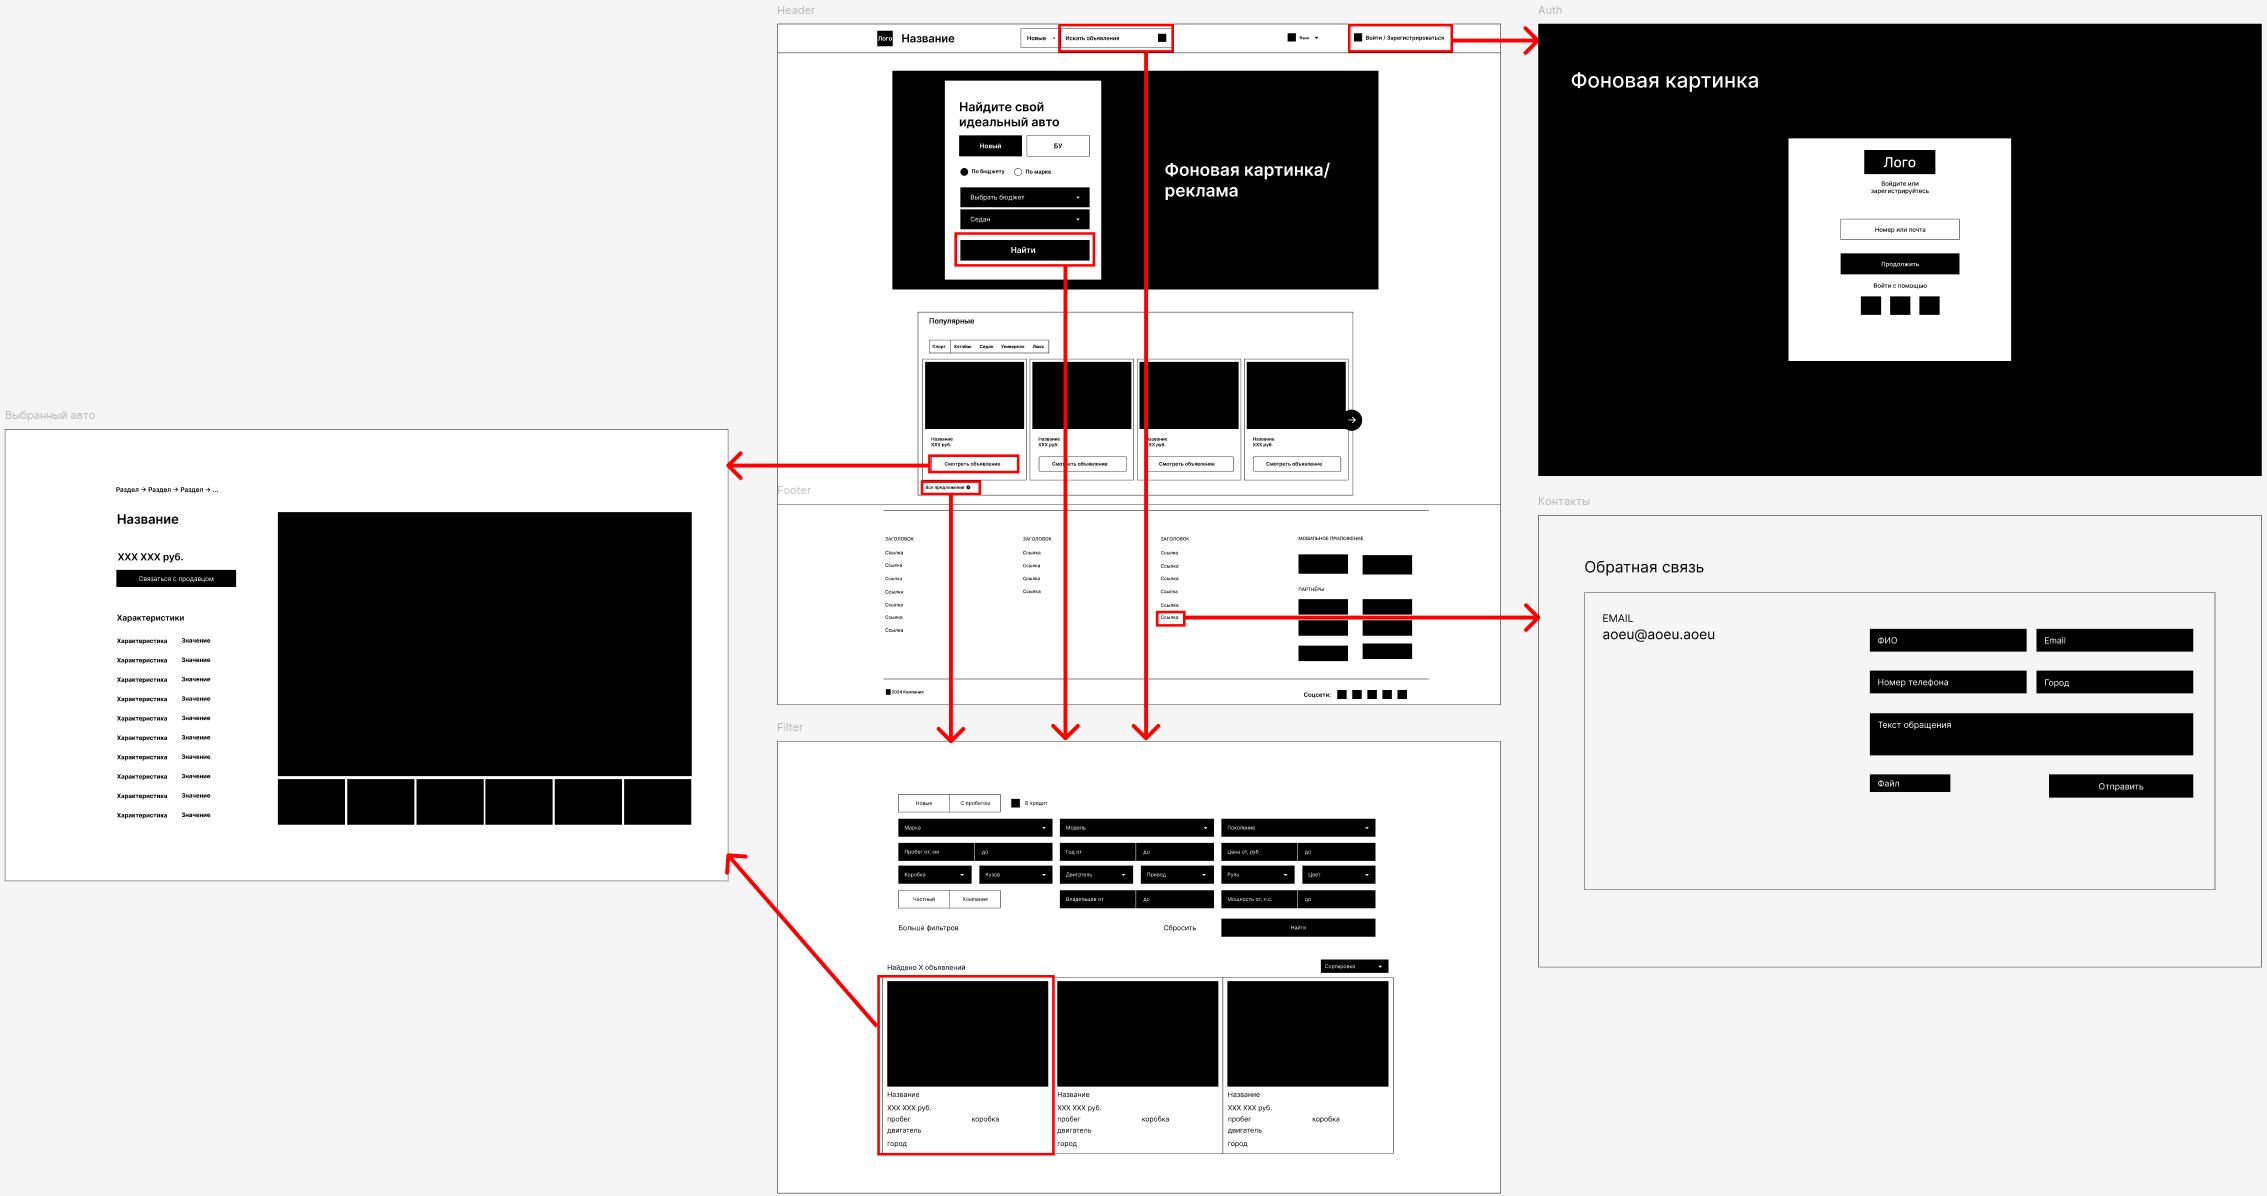
\includegraphics[width=\linewidth]{wireflow}}
    \captionof{figure}{Wireflow}
\end{minipage}
\bigskip

\textbf{Контрольные вопросы и ответы}

\begin{enumerate}
    \item Что такое Wire flow?

Wire flow — это комбинация блок-схемы и каркасов (wireframes), которая документирует рабочий процесс и дизайн экрана, особенно когда имеется несколько динамически меняющихся страниц. Он показывает, как пользователь взаимодействует с элементами интерфейса на пути к достижению своей цели.
    \item Какое место при проектировании интерфейсов занимает создание Wire flow?

Создание Wire flow занимает важное место в проектировании интерфейсов, так как оно помогает визуализировать и структурировать взаимодействие между элементами на экранах. Это позволяет уточнить техническое задание и улучшить понимание пользовательского опыта до начала этапа тестирования.
    \item Где используются Wire flow? Назначение

Wire flow используется в проектировании мобильных приложений, веб-сайтов и настольных продуктов. Его назначение заключается в документировании и визуализации взаимодействия пользователя с интерфейсом, а также в упрощении процесса разработки и тестирования.
    \item Какие программные средства используются для создания Wire flow?

Для создания Wire flow используются различные программные средства, такие как Miro, Figma, Flowmapp, Sketch, а также онлайн-сервисы, такие как draw.io и Lucidchart. Эти инструменты позволяют создавать визуальные схемы и макеты, упрощая процесс проектирования.
\end{enumerate}

\end{document}
